% -----------------------------------------------
% Template for ISMIR Papers
% 2015 version, based on previous ISMIR templates
% -----------------------------------------------

\documentclass{article}
\usepackage{ismir,amsmath,cite}
\usepackage{graphicx}
\usepackage{color}

% Title.
% ------
\title{Paper Template For ISMIR \conferenceyear}


% Single address
% To use with only one author or several with the same address
% ---------------
%\oneauthor
% {Names should be omitted for double-blind reviewing}
% {Affiliations should be omitted for double-blind reviewing}

% Two addresses
% --------------
%\twoauthors
%  {First author} {School \\ Department}
%  {Second author} {Company \\ Address}

% Three addresses
% --------------
\threeauthors
  {First author} {Affiliation1 \\ {\tt author1@ismir.edu}}
  {Second author} {\bf Retain these fake authors in\\\bf submission to preserve the formatting}
  {Third author} {Affiliation3 \\ {\tt author3@ismir.edu}}

% Four addresses
% --------------
%\fourauthors
%  {First author} {Affiliation1 \\ {\tt author1@ismir.edu}}
%  {Second author}{Affiliation2 \\ {\tt author2@ismir.edu}}
%  {Third author} {Affiliation3 \\ {\tt author3@ismir.edu}}
%  {Fourth author} {Affiliation4 \\ {\tt author4@ismir.edu}}

\begin{document}
%
\maketitle
%
\begin{abstract}
The abstract should be placed at the top left column and should contain about 150-200 words.
\end{abstract}
%
\section{Introduction}\label{sec:introduction}

	This template includes all the information about formatting manuscripts for the ISMIR \conferenceyear\ Conference.
	Please follow these guidelines to give the final proceedings a uniform look.
	Most of the required formatting is achieved automatically by using the supplied
	style file (\LaTeX) or template (Word).
	If you have any questions, please contact the Program Committee
	(\texttt{ismir\conferenceyear-papers@ismir.net}).
	This template can be downloaded from the ISMIR \conferenceyear\ web site (\texttt{http://ismir\conferenceyear.ismir.net}).
	%
	\section{Paper Length}
	\textcolor{red}{The regulations for the maximal paper length have changed.}
	Instead of the strict limit of six pages (as used for ISMIR 2014), we adopt 
	a ``(6+1)-page policy'' for ISMIR 2015. This means, the paper may have a 
	maximum of 6 pages for technical content including figures and possible references 
	with one additional optional 7th page containing only references.
	Note that this is a strict requirement. 
	\textcolor{red}{The seventh page (if used at all) must
	not contain any other material except for references.}

\section{Short Fast Fourier Transform (SFFT)}\label{sec:sfft}

	A transformada discreta de fourier (DFT ou  FFT) é muito utilizada para a construcao das caracteristicas cromaticas (chroma feature) do audio. A funcao dessa transformada eh traduzir informacoes que estao em dominio temporal para dominio frequencial de tal forma a projetar, em bases ortonormais, o valor de cada componente senoidal presente no sinal tratado. Essa projecao se da pelo somatorio do produto interno das senoides (exponenciais complexas) pelo sinal.

	Visto que essa transformada somente oferece informacoes em termos de frequencias, surgiu-se a necessidade de adapta-la para a visualizacao das variacoes das frequencias ao longo do tempo. Essa adaptacao se denomina transformada de fourier janelada (SFFT). Esse processo de janelamento se resume a dividir o sinal em partes, para serem analisadas individualmente no domínio da frequência, ou seja, a cada instante de tempo referente a cada trecho eh possivel obter uma analise frequencial.

	Porem essa tecnica possui as seguintes limitacoes:
	\begin{itemize}
		\item surgimento de frequencias fantasmas (alising) que podem dificultar a identificacao das notas musicais que foram verdadeiramente tocadas;
		\item problemas de vazamento gerados pelo truncamento do sinal, podendo gerar frequencias que dificultam a visualizacao do espectro (leakage);
		\item dificuldades na determinacao do tamanho da janela pois trata-se de um parametro de amostragem que pode limitar a banda de frequencia a ser analisada.
	\end{itemize}


\section{Chroma Convolution Method (CCM)}\label{sec:ccm}

	Em vista das limitações apresentadas da SFFT, foi desenvolvido um metodo no dominio do tempo que preserva as caracteristicas originais do sinal. O chroma convolution method (CCM) objetiva a projecao dos trechos do sinal sobre cada um dos sinais das notas musicais procuradas. Observa-se que quando o trecho do sinal eh projetado sobre o sinal de uma nota musical, atraves da convolucao, esta nota eh amplificada e as demais são suprimidas.

	Seja uma nota musical formada a partir de uma senoide monocromatica. Quando esse sinal eh convoluido com um trecho de sinal de audio eh possivel extrair como resultado o nivel de energia relacionado a esta frequencia. Tal energia eh mensurada a partir da seguinte equacao \eqnref{ccm_equation}:

	\begin{equation}\label{ccm_equation}
		E = \sum [f(x)*g(x)]^{2}
	\end{equation}

	Neste contexto as caracteristicas cromaticas (chroma feature) foram construidas a partir dos seguintes procedimentos:
	\begin{enumerate}
		\item dividiu-se o audio a ser analisado em sinais com duracao pre-determinada;
		\item funcoes senoidais monocromaticas foram utilizadas para construir notas musicais no dominio do tempo, correspondendo a escala cromatica musical; 
		\item convoluiu-se cada parte do sinal do sinal de audio com as notas musicais;
		\item a energia da convolucao foi extraida a partir da equacao \eqnref{ccm_equation};
		\item por fim cada energia foi somada com suas respectivas oitavas, originando o chroma feature.
	\end{enumerate}

	A figura abaixo representa uma visao esquematica do procedimento descrito. Ao final do processo as caracteristicas cromaticas (chroma feature) podem ser visualizadas a partir de um espectrograma.

	\begin{figure}[h]
	 \centerline{\framebox{
	 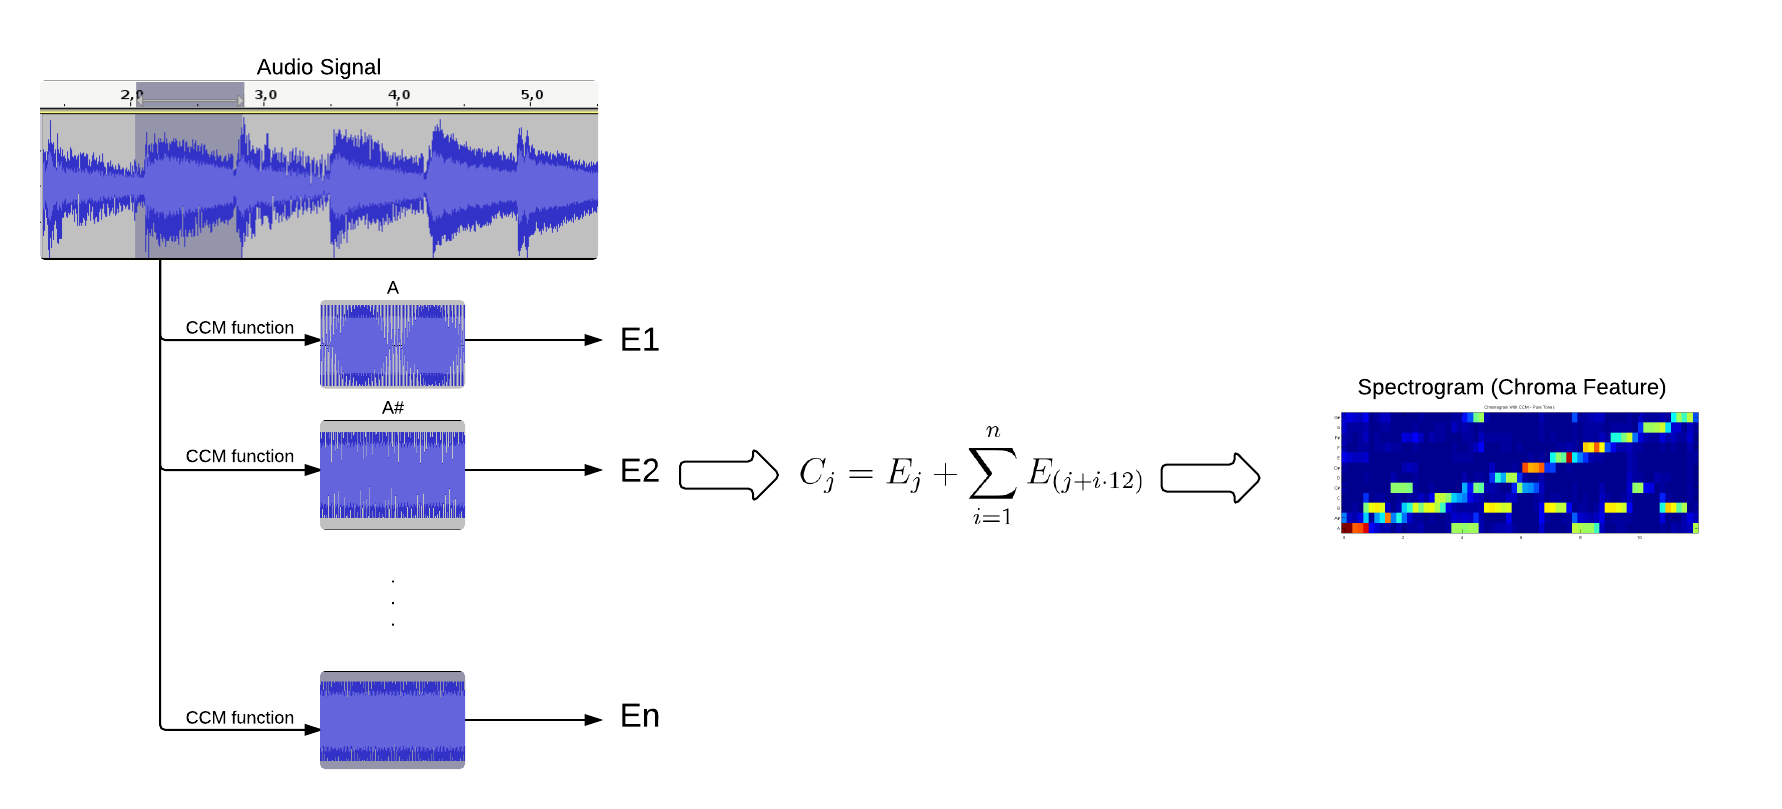
\includegraphics[width=\columnwidth]{figs/schematic.png}}}
	 \caption{Schematic of process to build chroma feature using CCM.}
	 \label{fig:schematic}
	\end{figure}


\section{Experiments and Results}

	Com o intuito de demonstrar a eficacia do CCM em relacao ao tradicional metodo SFFT\cite{LabROSA} no que diz respeito identificacao das notas tocadas a partir de suas caracteristicas cromaticas (chroma feature),  foram realizados 2 experimentos usando a linguagem de programacao MATLAB. Como entrada de dados usou-se sinais de audio gravados por instrumentos musicais reais\footnote{Code and files available in https://github.com/josepedro/ismir\_article.}. 

	\subsection{Experiment 1: Identification of Musical Notes}

	O primeiro experimento se trata de identificacao de notas musicais numa melodia de piano. Tais notas foram tocadas segundo a \figref{fig:1-notes}: 

	\begin{figure}[h]
	 \centerline{\framebox{
	 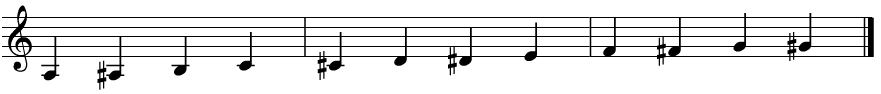
\includegraphics[width=\columnwidth]{figs/1-notes.png}}}
	 \caption{Notes that were played and recorded on piano.}
	 \label{fig:1-notes}
	\end{figure}

	Utilizou-se convolucao com 96 tons puros de diferentes frequencias para gerar o chroma feature. As janelas de ambas as propostas foram configuradas no tamanho de 0.120 segundos e a taxa de amostragem do audio foi de 44.1 kHz.

	\subsubsection{SFFT Results}
	Segue chroma feature encontrado utilizando o metodo tradicional da SFFT em \figref{fig:1-ssft}. Observa-se que a escala cromatica foi identificada, porem com erros em relacao ao momento exato em que as notas foram tocadas. Nota-se, por exemplo, que uma nota E foi identificada no comeco quando na verdade deveria ter sido identificada nos instantes proximos de 7 segundos.

	
	\begin{figure}[h]
	 \centerline{\framebox{
	 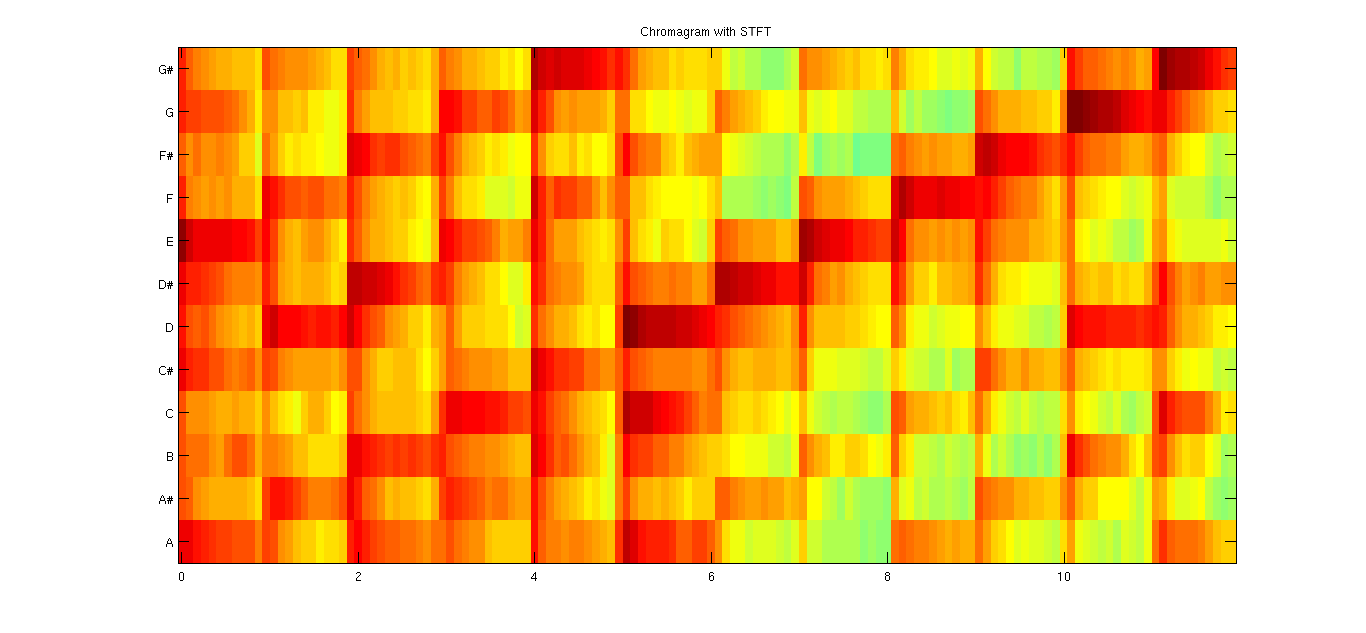
\includegraphics[width=\columnwidth]{figs/1-sfft.png}}}
	 \caption{Chroma feature of audio using SFFT.}
	 \label{fig:1-ssft}
	\end{figure}	

	\newpage
	Foi tambem feito uma analise de eficiencia das notas gravadas no audio com a sequencia de notas identificas no chroma feature. As notas identificadas foram selecionadas atraves da maior intensidade em cada instante de tempo. Segue tabela comparativa:

	\begin{table}[h]
	 \begin{center}
	 \begin{tabular}{|l|l|}
	  \hline
	  Played Notes & Identified Notes \\
	  \hline
	  A  & E \\
	  A\#  & D \\
	  A\#  & D\# \\
	  B  & B \\
	  B\#  & E \\
	  C  & D \\
	  C\#  & G\# \\
	  D  & D \\
	  D\#  & D\# \\
	  E  & E \\
	  F  & F \\
	  F\#  & F\# \\
	  G  & G \\
	  G\#  & G\# \\
	  \hline
	 \end{tabular}
	\end{center}
	 \caption{Comparison between played notes and identified notes.}
	 \label{tab:table-1-sfft}
	\end{table}

	Dado os dados da tabela \tabref{tab:table-1-sfft}, houve 9 de 14 notas tocadas em instantes corretos, ou seja, 64.2857\% de fidelidade com a melodia original.


	\subsubsection{CCM Results}
	Segue chroma feature encontrado utilizando o CCM:
	
	\begin{figure}[h]
	 \centerline{\framebox{
	 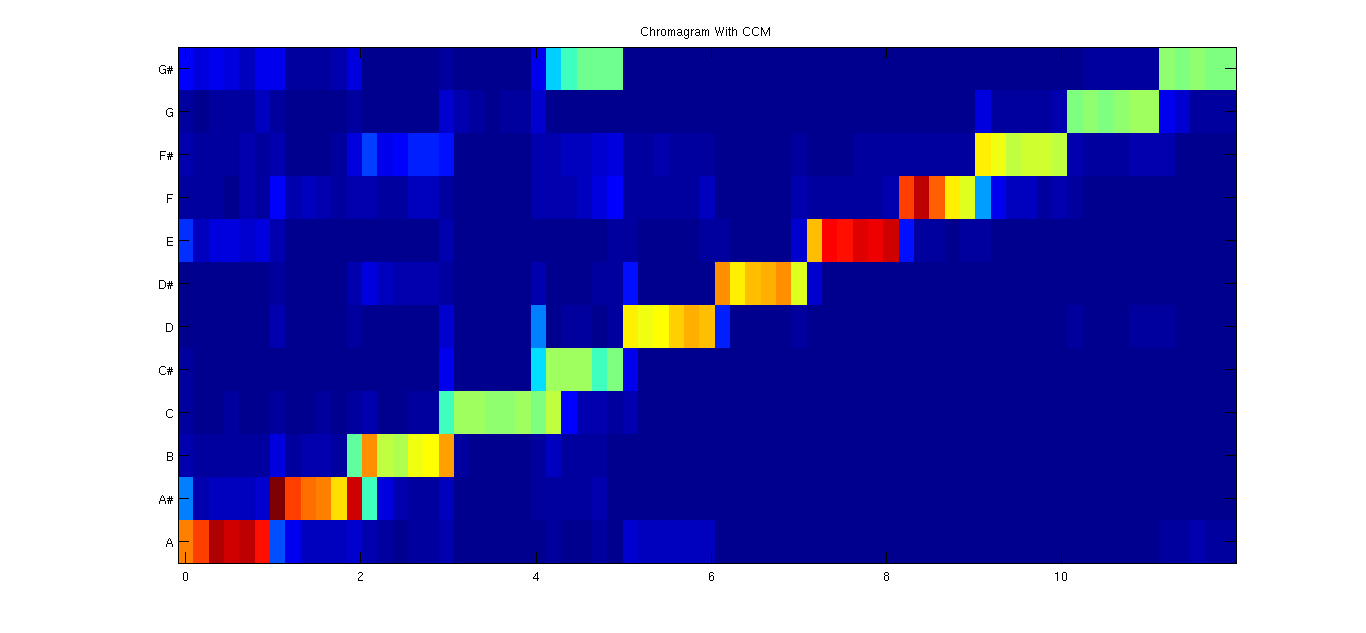
\includegraphics[width=\columnwidth]{figs/1-ccm.png}}}
	 \caption{Chroma feature of audio using CCM.}
	 \label{fig:1-ccm}
	\end{figure}	


	Observa-se na figura \figref{fig:1-ccm} que a melodia apresentou uma maior clareza. Uma tabela comparativa das notas tocadas e identificadas foi feita tambem atraves da estrategia dos maximos:

	\begin{table}[h]
	 \begin{center}
	 \begin{tabular}{|l|l|}
	  \hline
	  Played Notes & Identified Notes \\
	  \hline
	  A  & A \\
	  A\#  & A\# \\
	  B  & B \\
	  C  & C \\
	  C\#  & C\# \\
	  C\#  & G\# \\
	  C\#  & C\# \\
	  D  & D \\
	  D\#  & D\# \\
	  E  & E \\
	  F  & F \\
	  F\#  & F\# \\
	  G  & G \\
	  G\#  & G\# \\
	  \hline
	 \end{tabular}
	\end{center}
	 \caption{Comparison between played notes and identified notes from chroma feature.}
	 \label{tab:table-1-ccm}
	\end{table}

	Em vista dos resultados de \tabref{tab:table-1-ccm}, houve 13 de 14 notas tocadas em instantes corretos, ou seja, 92.8571\% de fidelidade com a melodia original.


	\subsection{Experiment 2: Identification of Musical Notes of Different Instruments}

	O segundo experimento diz respeito a identificação de notas musicais de diferentes instrumentos. Para tal foram tocadas as seguintes melodias no piano e violao juntas:

	\begin{figure}[h]
	 \centerline{\framebox{
	 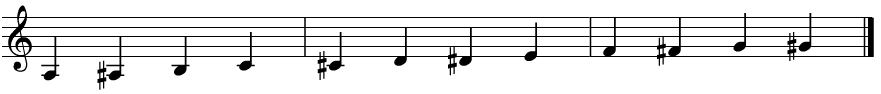
\includegraphics[width=\columnwidth]{figs/1-notes.png}}}
	 \centerline{\framebox{
	 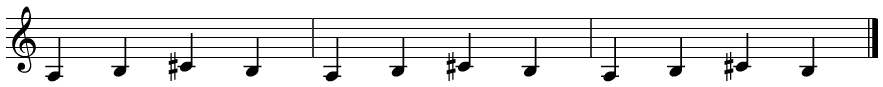
\includegraphics[width=\columnwidth]{figs/2-notes-violao.png}}}
	 \centerline{\framebox{
	 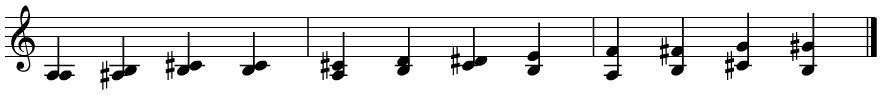
\includegraphics[width=\columnwidth]{figs/2-notes-violao-piano.png}}}
	 \caption{The first sheet music is only piano, the second sheet music is only acoustic guitar and the third sheet music is the both together.}
	 \label{fig:1-ssft}
	\end{figure}

Utilizou-se convolucao com 12 tons de violao e 12 tons de piano de diferentes frequencias gerando dois chroma feature respectivamente, um para cada instrumento. As janelas de ambas as propostas foram configuradas no tamanho de 0.120 segundos e a taxa de amostragem do audio foi de 44.1 kHz.

	\subsubsection{SFFT Results}
	Segue chroma feature encontrado utilizando o metodo tradicional da SFFT:
	
	\begin{figure}[h]
	 \centerline{\framebox{
	 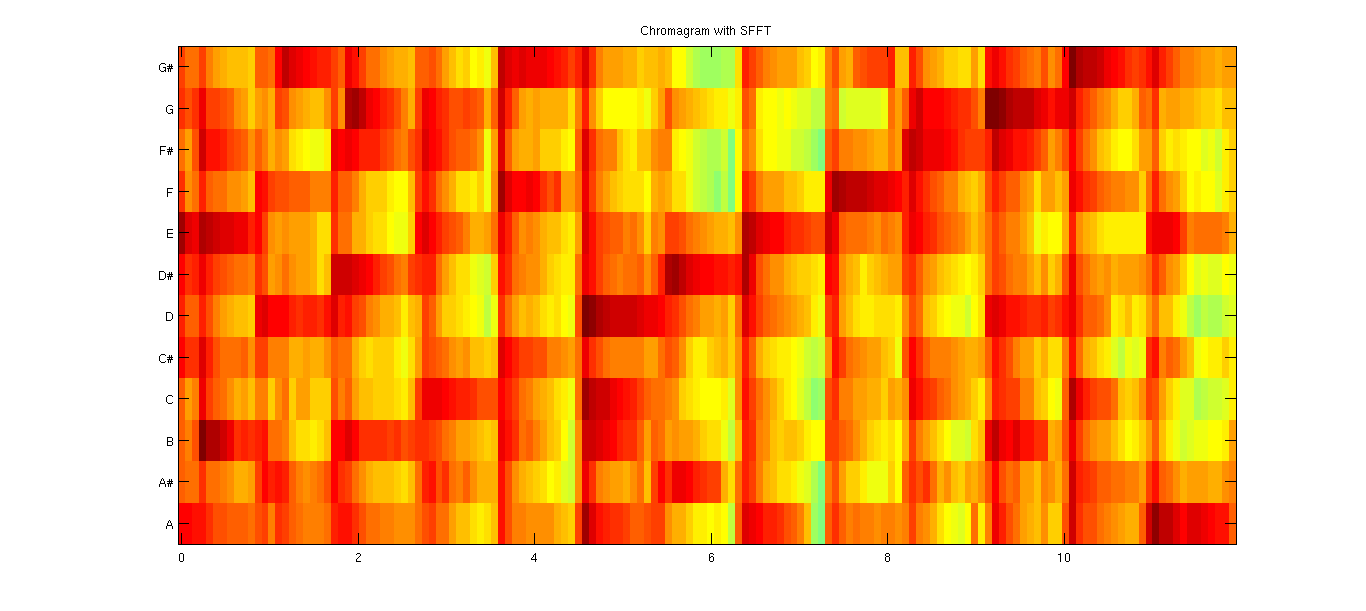
\includegraphics[width=\columnwidth]{figs/2-sfft.png}}}
	 \caption{Chroma feature of audio using SFFT.}
	 \label{fig:2-ssft}
	\end{figure}	

	Observa-se na figura \figref{fig:2-ssft} que a escala cromatica do piano foi parcialmente identificada. As notas do violao sao praticamente imperceptiveis.

	Foi tambem feito uma analise de eficiencia das notas gravadas dos dois instrumentos com a sequencia de notas identificadas no chroma feature, usando a maior intensidade em cada instante de tempo. Segue tabela comparativa:

	\begin{table}[h]
	 \begin{center}
	 	\centerline{
	 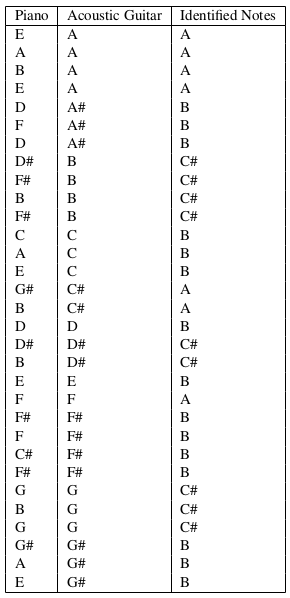
\includegraphics[width=\columnwidth,height=12cm]{figs/tabela_2.png}}
	 \end{center}
	 \caption{Comparison between played notes of piano, acoustic guitar and identified notes of chroma feature.}
	 \label{tab:table-2-sfft}
	\end{table}

	Segundo os dados da tabela \tabref{tab:table-2-sfft}, houve 12 de 31 notas de piano tocadas em instantes corretos, ou seja, 38.7096\% de fidelidade com a melodia original do piano. Quanto ao violao, somente 1 nota foi tocada em instante certo, ou seja, 3.2258\% de fidelidade com a melodia original do violao.

%-------------------------------------------------------------------
	\subsubsection{CCM Results}
	Segue chroma feature encontrado utilizando o CCM de tons de piano:
	
	\begin{figure}[h]
	 \centerline{\framebox{
	 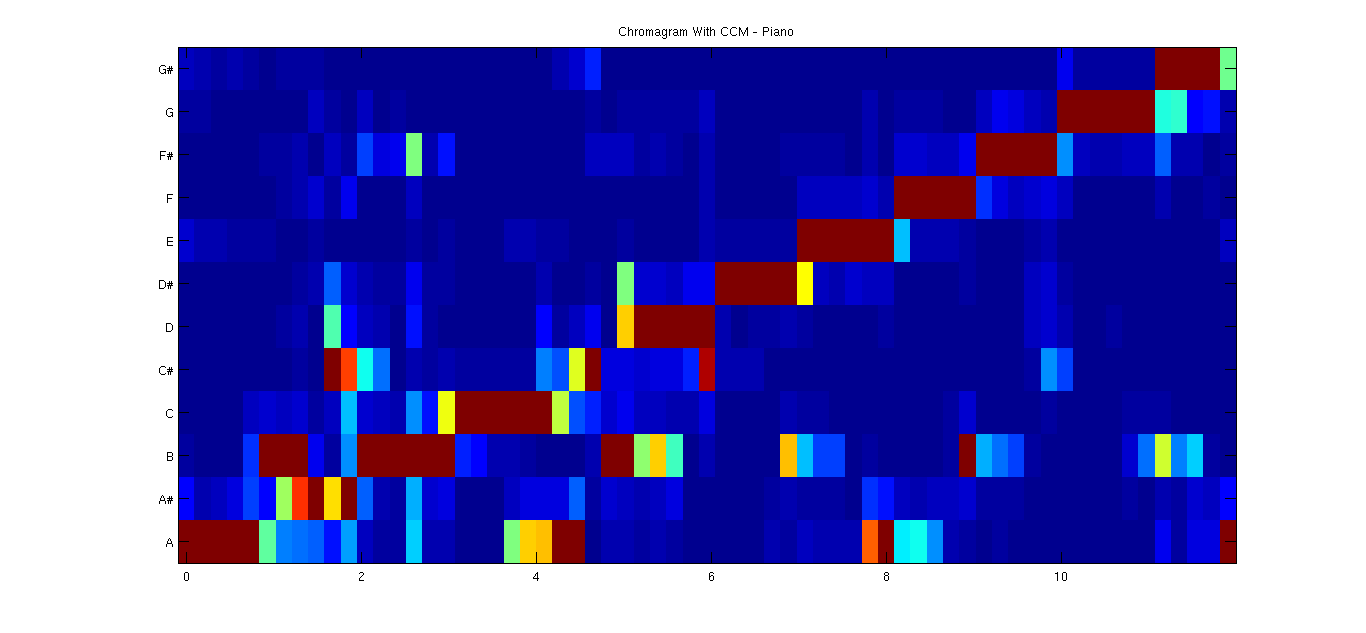
\includegraphics[width=\columnwidth]{figs/2-ccm-piano.png}}}
	 \caption{Chroma feature of audio using CCM of piano tones.}
	 \label{fig:2-ccm-piano}
	\end{figure}	

	Observa-se na figura \figref{fig:2-ccm-piano} que a melodia apresentou uma maior clareza. Eh visivel tambem a escala cromatica tocada pelo piano e algumas poucas notas do violao. Uma tabela comparativa das notas tocadas identificadas foi feita tambem atraves da estrategia dos maximos:

	\begin{table}[h]
	 \begin{center}
	 \begin{tabular}{|l|l|l|}
	  \hline
	  Piano & Acoustic Guitar & Identified Notes \\
	  \hline
		A	& A	& A \\
		A	&    B	&    B \\
		A\#	&    B	&    A\# \\
		A\#	&    B	&    C\# \\
		A\#	&    C\#	&    A\# \\
		B	&    B	&    B \\
		C	&    A	&    C \\
		C\#	&    A	&    A \\
		C\#	&    B	&    C\# \\
		D	&    B	&    B \\
		D	&    C\#	&    D \\
		D\#	&    B	&    D\# \\
		E	&    A	&    E \\
		F	&    B	&    F \\
		F\#	&    C\#	&    F\# \\
		G	&    B	&    G \\
		G\#	&    B	&    G\# \\
		G\#	&    B	&    A \\
	  \hline
	 \end{tabular}
	\end{center}
	 \caption{Comparison between played notes of piano, acoustic guitar and identified notes of chroma feature with piano tones.}
	 \label{tab:table-2-ccm-piano}
	\end{table}

	
	Em vista dos resultados de \tabref{tab:table-2-ccm-piano}, houve 13 de 18 notas de piano em instantes corretos, ou seja, 72.2222\% de fidelidade com a melodia original. Quanto ao violao, houve 5 de 18 notas em instantes corretos, ocasionando em 27.7777\%. Tal resultado mostra que o CCM usando tons de piano realmente amplificou as suas notas e suprimiu as do violao.



Segue chroma feature encontrado utilizando o CCM de tons de violao:
	
	\begin{figure}[h]
	 \centerline{\framebox{
	 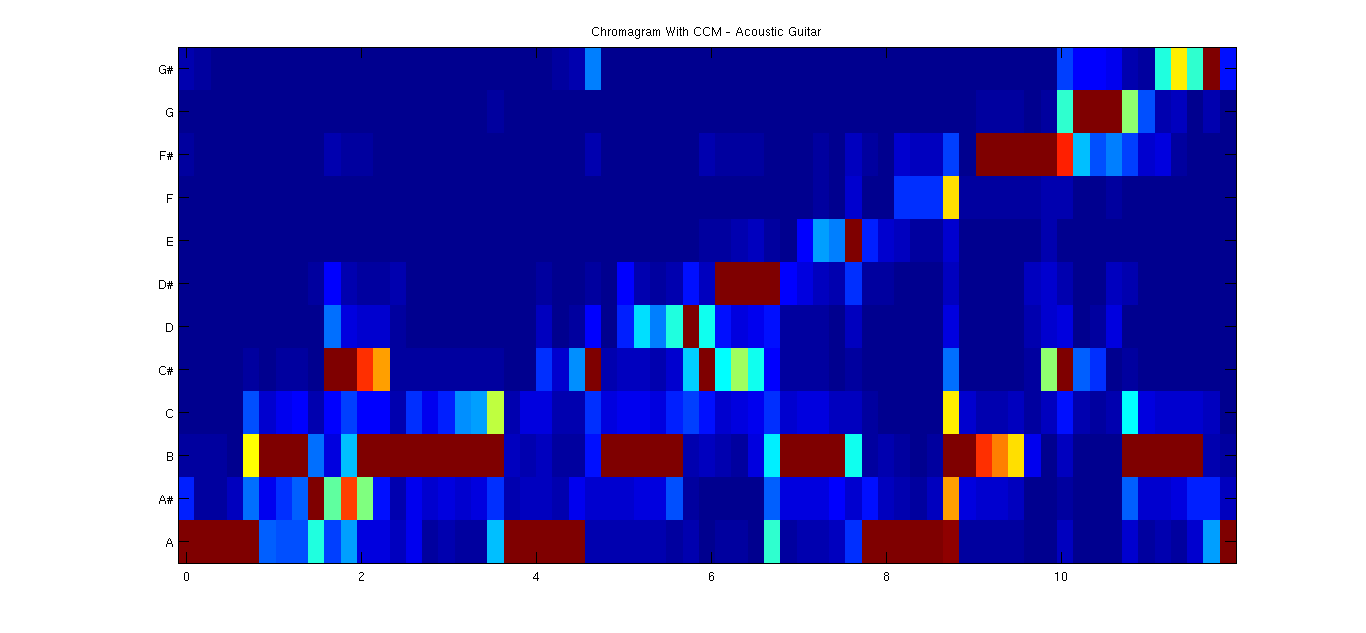
\includegraphics[width=\columnwidth]{figs/2-ccm-violao.png}}}
	 \caption{Chroma feature of audio using CCM of acoustic guitar tones.}
	 \label{fig:2-ccm-violao}
	\end{figure}	

	Observa-se na figura \figref{fig:2-ccm-violao} que a melodia apresentou uma maior clareza. Eh visivel tambem a escala cromatica tocada pelo piano suprimida e as notas do violao amplificadas. Uma tabela comparativa das notas tocadas e identificadas foi feita tambem atraves da estrategia dos maximos:

	\begin{table}[h]
	 \begin{center}
	 \begin{tabular}{|l|l|l|}
	  \hline
	  Piano & Acoustic Guitar & Identified Notes \\
	  \hline
			  A & A &  A \\
		A\# &  B &  B \\
		    A\# &  B &    A\# \\
		    B  &   C\# &  C\# \\
		    C   &  B  &   B \\
		    C\# &  A   &  A \\
		    D   &  B   &  C\# \\
		    D\# &  C\# &  B \\
		    D\# &  C\# &  D \\
		    D\# &  C\# &  C\# \\
		    E   &  B  &   D\# \\
		    F   &  A   &  B \\
		    F   &  A  &   E \\
		    F\# &  B  &   A \\
		    F\# &  B   &  B \\
		    G   &  C\# &  F\# \\
		    G   &  C\# &  C\# \\
		    G\# &  B   &  G \\
		    G\# &  B  &   B \\
	  \hline
	 \end{tabular}
	\end{center}
	 \caption{Comparison between played notes and identified notes.}
	 \label{tab:table-2-ccm-violao}
	\end{table}

	\newpage
	Em vista dos resultados de \tabref{tab:table-2-ccm-violao}, houve 9 de 19 notas de violao em instantes corretos, ou seja, 47.3684\% de fidelidade com a melodia original. Quanto ao piano, houve 2 de 19 notas em instantes corretos, ocasionando em 10.5263\%. Tal resultado mostra que o CCM usando tons de violao realmente amplificou as suas notas e suprimiu as do piano.


\section{Discussion}\label{sec:discussion}

	Em vista dos resultados alcancados, ha limitacao e beneficios no uso da convolucao em relacao a transformada de fourier janelada. Uma limitacao encontrada foi o tempo de processamento que no metodo da SFFT foi de 0.100138 segundos enquanto no CCM foi de 13.266711 segundos para o primeiro experimento.

	Do ponto de vista dos beneficios, o primeiro experimento mostra que o CCM eh mais eficiente do que o SFFT para caracterizacao de notas. O SFFT obteve um rendimento de 64.2857\% enquanto que o CCM obteve 92.8571\%, ocasionando em 28.5714\% a mais de notas identificadas com o CCM. Tal fato se deve pela reducao de ruidos e intensificacao das frequências sonoras realmente gravadas pelo instrumento musical. 

	Do segundo experimento observa-se um beneficio muito importante no uso do CCM, a possibilidade de distinguir instrumentos musicais tocados juntos. Alem da SFFT nao possuir a possibilidade de geracao de um chroma feature para cada instrumento, ela gerou resultados baixos em comparacao com CCM na identificacao das melodias do piano (38.7096\%) e violao (3.2258\%).

	Usando o CCM gerou-se, para cada instrumento, um chroma feature. O chroma feature do piano possuiu identificacao de 72.2222\% de notas de melodia de piano e 27.7777\% de melodia de violao. Esse fato demonstra que o chroma feature do piano realmente destaca as suas notas de timbre caracteristico. O chroma feature do violao tambem possuiu tal capacidade com 47.3684\% de fidelidade para melodia do violao e 10.5263\% para melodia de piano. Eh notavel que o CCM possui um potencial maior de identificacao que o SFFT para ambos instrumentos alem de destacar mais diferentes instrumentos.


	\section{Conclusions and Future Works}\label{sec:conclusions}

	Em vista do que foi proposto, foi apresentado uma nova forma de construcao da chroma feature usando o chroma convolution method (CCM). Comparou-se o metodo proposto com o tradicional SFFT e o CCM mostrou-se mais satisfatorio. 

	A eficiencia do CCM frente ao SFFT nao foi somente pela deteccao de melodias monofonicas, mas tambem pela identificacao de melodias polifonicas com mais de um instrumento. O CCM possui a capacidade diferencial de trabalhar com timbres de instrumentos musicais para a dinstincao dos mesmos no audio.

	 Pode-se concluir que melhorias que foram feitas na forma simples da SFFT em trabalhos correlatos podem ser aplicadas no CCM, aumentando assim seu potencial. Tambem eh de significativa importancia demonstrar a otimizacao dos resultados de sistemas de transcricao automatica de acordes usando o CCM.

	Assim como ocorre na SFFT, é plausivel de implementacao de um pre-processamento de sinal utilizando filtros no CCM para a caracterizacao de instrumentos em audios mais complexos como o de uma banda ou orquestra.




% For bibtex users:
\bibliography{ISMIR2015template}

% For non bibtex users:
%\begin{thebibliography}{citations}
%
%\bibitem {Author:00}
%E. Author.
%``The Title of the Conference Paper,''
%{\it Proceedings of the International Symposium
%on Music Information Retrieval}, pp.~000--111, 2000.
%
%\bibitem{Someone:10}
%A. Someone, B. Someone, and C. Someone.
%``The Title of the Journal Paper,''
%{\it Journal of New Music Research},
%Vol.~A, No.~B, pp.~111--222, 2010.
%
%\bibitem{Someone:04} X. Someone and Y. Someone. {\it Title of the Book},
%    Editorial Acme, Porto, 2012.
%
%\end{thebibliography}

\end{document}
